\documentclass[letter, 10pt]{article}
\usepackage[utf8]{inputenc}
\usepackage[spanish, es-tabla]{babel}
\usepackage{amsfonts}
\usepackage{amsmath}
\usepackage[dvips]{graphicx}
\usepackage{graphicx}
\usepackage{subfigure} % subfiguras
\DeclareGraphicsExtensions{.bmp,.png,.pdf,.jpg}
\usepackage{xcolor,listings}%color support for listings
\usepackage{epstopdf}
\usepackage{algpseudocode}
\usepackage{algorithm}
\usepackage{url}
\usepackage{caption}
\usepackage{cite}
\usepackage[top=3cm,bottom=3cm,left=3.5cm,right=3.5cm,footskip=1.5cm,headheight=1.5cm,headsep=.5cm,textheight=3cm]{geometry}



\begin{document}



\title{Análisis Inteligente de Datos \\ \begin{Large}Tarea 2\end{Large}}
\author{Paulina Aguila - Juan Avalo}
\date{23 de junio de 2016}

\maketitle


\begin{figure}[ht]
\begin{center}

\includegraphics[width=0.2\textwidth]{Images/Isotipo-Negro.png}\\
\end{center}
\end{figure}
\vspace{2cm}

\section{Regresión Lineal Ordinaria (LSS)}

En esta sección, se estudiará un dataset llamado \textit{prostate-cancer}\cite{D}, que se utiliza a menudo con métodos de regresión. Los datos corresponden a un estudio realizado por Tom Stamey (Universidad de Stanford) en 1989 referente a la posible correlación entre el nivel de antígeno prostático específico (PSA) medido en un paciente, y otras mediciones clínicas que se obtuvieron luego de extirpar totalmente la próstata y los tejidos circundantes. Una de las variables que se estudian corresponden al volumen del cáncer prostático detectado en el paciente.

\subsection{Descripción de los datos}
En base al dataset, se construye con Python un dataframe de dimensión (97,9), es decir, de 9 variables y 97 datos. A continuación, se describen las variables \cite{DD}:

\begin{itemize}
\item \textbf{Lcavol: }Variable cuantitativa continua que representa el registro del volumen del cáncer. Toma valores flotantes desde -1,347 hasta 3,821.
\item \textbf{Lweight: }Variable cuantitativa continua que registra el valor del peso de la próstata. Toma valores flotantes desde 2,375 hasta 4,780. 
\item \textbf{Age: }Variable cuantitativa de tipo continua que representa la edad en años de la persona. Toma valores enteros desde 41 hasta 79 años.
\item \textbf{Lbph: }Variable cuantitativa continua que registra la cantidad de hiperplasia prostática benigna (HBP)\footnote{La hiperplasia benigna de próstata (HBP) es un agrandamiento no canceroso de la glándula prostática cuya prevalencia aumenta progresivamente con la edad.}. Toma valores flotantes desde -1,386 hasta 2,326. 
\item \textbf{Svi: }Variable categórica binaria que representa si existe invasión del cáncer en la vesícula seminal\footnote{Las vesículas o glándulas seminales son las encargadas de producir el 60\% del volumen del líquido seminal. Están ubicadas por encima de la base de la próstata, con la que están unidas por su extremo inferior.}. Toma los siguientes valores: 0: No hay invasión - 1: Si hay invasión. 
\item \textbf{Lcp: }Variable cuantitativa de tipo continua que representa el registro de penetración capsular\footnote{La próstata posee una fina envoltura que se conoce como cápsula prostática que define su límite. La penetración capsular es cuando las células cancerígenas se extienden y cruzan dicha envoltura.}. Toma valores flotantes entre -1,386 y 2,904. 
\item \textbf{Gleason: }Variable categórica ordinal que contiene el puntaje de Gleason\footnote{La escala de Gleason es un sistema que se emplea para medir el grado de agresividad de un cáncer de próstata, basándose en la observación de una muestra de biopsia. Si toma valores entre 2 y 6 corresponde a un cáncer con escasa agresividad, si toma valor 7 es un cáncer con agresividad intermedia, mientras que, si es de 8 a 10, corresponde a un cáncer de alta agresividad y peor pronóstico.}. Toma valores enteros entre 6 y 9.
\item \textbf{Pgg45: }Variable cuantitativa continua que representa el porcentaje del patrón de Gleason 4 y 5\footnote{El porcentaje del patrón de Gleason 4/5 se obtiene agregando los porcentajes de los patrones 4 y 5 de Gleason, es decir, la proporción combinada del tumor compuesto por el patrón 4 o el patrón 5 de Gleason, o ambos.}. Toma valores enteros entre 0 y 100.
\item \textbf{Lpsa: }Variable cuantitativa continua que corresponde al registro del análisis del antígeno prostático específico (PSA)\footnote{El antígeno prostático específico, o PSA, es una proteína producida por las células de la glándula prostática. El análisis del PSA mide la concentración del PSA en la sangre de un hombre. La concentración del PSA en la sangre es frecuentemente elevada en hombres con cáncer de próstata.}. Toma valores flotantes entre -0,430 hasta 5,583.
\item \textbf{Train: }Variable categórica nominal que representa si el dato es de tipo Test o de Training. Del total de 97 datos, 67 de ellos corresponden a datos de entrenamiento, mientras que 30 son datos de prueba. Toma los siguientes valores: T: Training set - F: Test set.
\end{itemize}

\subsection{Desarrollo}
Para comenzar con el desarrollo de la regresión lineal, en primer lugar, se deben normalizar los datos. Este es un paso muy importante, ya que permite ajustar la escala de las variables a la varianza de la unidad, lo que hace que los valores de datos que se encuentran ubicados en los extremos, no ejerzan un peso excesivo en la función objetivo.\\

Luego, al dataset se le debe quitar la columna \textbf{lpsa}, ya que esta formaría el vector y que corresponde a la función que se desea predecir. Al último dataframe, se le inserta una nueva columna llamada \textbf{intercept} compuesta solo de unos. Esto se realiza para que el modelo (ecuación) tenga un desplazamiento constante, el que actúa como intercepción \cite{P2}. Además, si se realiza el ajuste sin esa columna de unos, puede ocurrir que el coeficiente de determinación ($R^2$) pueda ser menor que cero. Es fácil de entender: puede que los regresores ensayados no den cuenta de la variabilidad de $\vec{y}$, y $SSE$ sea por tanto grande. Si acontece que $\vec{y}$ tiene poca variabilidad en torno a su media, $SST$ será en cambio pequeño, y $SST-SSE$ puede fácilmente ser negativo \cite{P1}.\\

Luego, de realizar estos pasos, se realiza una regresión lineal de mínimos cuadrados básica, para la cual se obtienen los valores del z-score y los pesos para cada variable. Para el cálculo del z-score, se realiza lo siguiente:

\begin{equation}
z_j=\frac{\hat{\beta}_j}{\hat{\sigma }\sqrt{v_j}}
\end{equation}

En donde, $\hat{\beta }_j$ son los coeficientes estimados por la regresión lineal del atributo $j$, $\hat{\sigma }$ corresponde a la desviación estándar estimada y $v_j$ es el $j$-ésimo elemento de $\left ( X^{T}X \right )^{-1}$. El iterador $j$ recorre todo el universo de atributos, por lo que en este caso $j=1,2,...,9$. La Tabla \ref{zscore} muestra un resumen con los valores obtenidos para cada variable.

\begin{table}[!hbt] 
\begin{center}
\begin{tabular}{| c | r | r |} 
\hline
\textbf{Variable} & \textbf{Peso} & \textbf{Z Score}\\ 
\hline 
lcavol & 0.676 & 5.319\\ 
lweight &0.261 & 2.727\\
age &-0.141 & -1.384\\
lbph &0.209 & 2.038\\
svi & 0.304& 2.448\\
lcp & -0.287& -1.851\\
gleason & -0.021& -0.145\\
pgg45 &0.266 &  1.723\\
intercept &2.465 & 27.359\\
\hline 
\end{tabular}
\caption{Recuadro con los coeficientes (pesos) y el valor del Z Score para cada variable.} 
\label{table:zscore}
\end{center} 
\end{table}

Dada la Tabla \ref{zscore}, se puede saber qué variables están más correlacionadas con la respuesta en base al valor que toma Z-Score, ya que las variables que tienen los mayores valores en valor absoluto del Z-Score, son las que más importancia y correlación tienen, por lo que son las que se deben seleccionar. En este caso, las variables más significativas por orden de importancia serían \textbf{lcavol}, \textbf{lweight}, \textbf{svi} y \textbf{lbph}. Esto tiene mucho sentido, ya que \textbf{lcavol} corresponde al volumen del cáncer, por lo que mientras más grande sea, mayor es la probabilidad de que tenga más PSA en la sangre. Al existir un Z-Score mayor que 2 en valor absoluto, esto quiere decir que la variable es significativa al nivel del 5\%, por lo que las variables menores a 2, como son \textbf{age}, \textbf{lcp}, \textbf{gleason} y \textbf{pgg45}.\\

Luego, se aplica Validación Cruzada o \textit{Cross Validation} con 5 y 10 bloques (k-folds) sobre los datos de entrenamiento, esto quiere decir, que los datos se dividen en 5 o 10 cajas. Para esto, es necesario realizar el ajuste de regresión lineal cada vez que se cambia el número de folds para que la estimación sea razonable. La Tabla \ref{msecross} muestra un resumen de los errores de predicción obtenidos.

\begin{table}[!hbt] 
\begin{center}
\begin{tabular}{| l | c |} 
\hline
\textbf{Set} & \textbf{Error}\\ 
\hline 
Test & 0.521\\ 
Training k=5 &0.957\\
Training k=10 &0.757\\
\hline 
\end{tabular}
\caption{Resumen con los errores de predicción para datos de test y training con validación cruzada.} 
\label{table:msecross}
\end{center} 
\end{table}

De la Tabla \ref{msecross}, se puede observar que para los datos de entrenamiento mientras más cantidad de bloques se utilicen en la validación cruzada, menor será el error de predicción obtenido, pero así mismo también aumentará la complejidad del algoritmo, dado que, si se aumenta la cantidad de k de tal forma que sea del mismo tamaño que la cantidad de datos, se obtendrá un error muy similar al real sin validación cruzada. Por otra parte, si se analiza el error del conjunto de prueba, se ve que el error es mucho menor. Este efecto se debe a la falta de regularización, ya que en validación cruzada se puede producir subajuste (underfitting) o sobreajuste (overfitting).\\

Se realiza un gráfico llamado ``quantile-quantile plot" para poder analizar si tiene sentido la hipótesis de que los residuos del modelo siguen una distribución normal. El gráfico se puede ver en la Figura \ref{qqplot}.

\begin{figure}[h]
\begin{center}
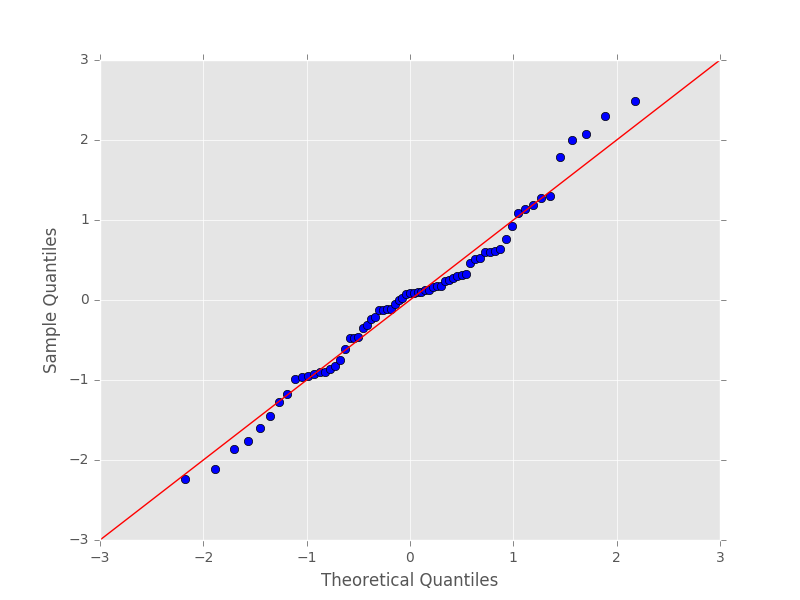
\includegraphics[width=0.7\textwidth]{Images/grafico1-j.png}
\caption{Histograma correspondiente a la cantidad de fallecidos y sobrevivientes de acuerdo a la variable edad.}
\label{qqplot}
\end{center}
\end{figure}

Del gráfico, se puede ver que sí se puede afirmar que tenga sentido que los residuos sigan una distribución normal, ya que los datos de la predicción (en azul), tienden a seguir la línea de los teóricos. Además, se observa que en el centro existe una tendencia que puede verse como una campana gaussiana.

\section{Selección de Atributos}

\subsection{Forward Step-wise Selection}

Usando el mismo dataframe anterior primero se ocupó el algoritmo de
\textit{Forward Step-wise Selection}(FSS) para selección de atributos. Dicho
algoritmo consiste en partir con un modelo lineal sin predictores, e ir
agregando uno por uno cada predictor, seleccionando el que tenga mejores
resultados de acuerdo a algún test dado. Luego de esa selección, se repite el
procedimiento con los atributos restantes hasta que quede un modelo con la
cantidad deseada de variables.\\

En la versión que se usó de base para hacer selección de atributos por FSS la
función usada para darle puntaje a cada variable era simplemente \textit{mean
  squared error}. De estos se seleccionaba el que diera menor error.

En la implementación presentada en éste trabajo se prefirió
usar el \textit{zscore} de cada variable. La razón de ésto es porque, para
elegir localmente una variable, basta ordenar el valor absoluto de los
\textit{zscore} de cada una de ellas y escoger el mayor de todos.

Para el análisis se va a ignorar la presencia del intercepto, la cual siempre se
selecciona.\\

Antes de comentar los resultados, hay que mencionar que la diferencia entre usar
\textit{mse} y \textit{zscore} no debiese ser muy distinta. En particular, se puede
analizar la función \textit{zscore}, definida como:
\begin{equation}
  z_j = \frac{\hat{\beta}_j}{\hat{\sigma}\sqrt{v_{j}}}
\end{equation}
Donde $\hat{\beta}_j$ es el coeficiente del modelo lineal $j$, $\hat{\sigma}$ es la
desviación estándar de los resultados del modelo, y $v_j$ es el componente
$j$-ésimo de la matriz $X^TX$.

Ésta función es más grande a medida que $\hat{\sigma}$ sea pequeño. $\hat{\sigma}$
es proporcional al \textit{mse} por lo que, manteniéndose todas las otras
variables igual, hace que ambas funciones tengan comportamientos similares al
momento de escoger. \\

Como resultado de aplicar \textit{FSS} se seleccionaron los atributos con el
siguiente orden:
\begin{enumerate}
\item Lcavol 
\item Lweigh
\item Svi
\item Lbph
\item Pgg45
\item Lcp
\item Age
\item Gleason   
\end{enumerate}

El gráfico que muestra el error de entrenamiento vs el error de test se
muestra a continuación:

\begin{figure}[H]
  \centering
<<<<<<< HEAD
 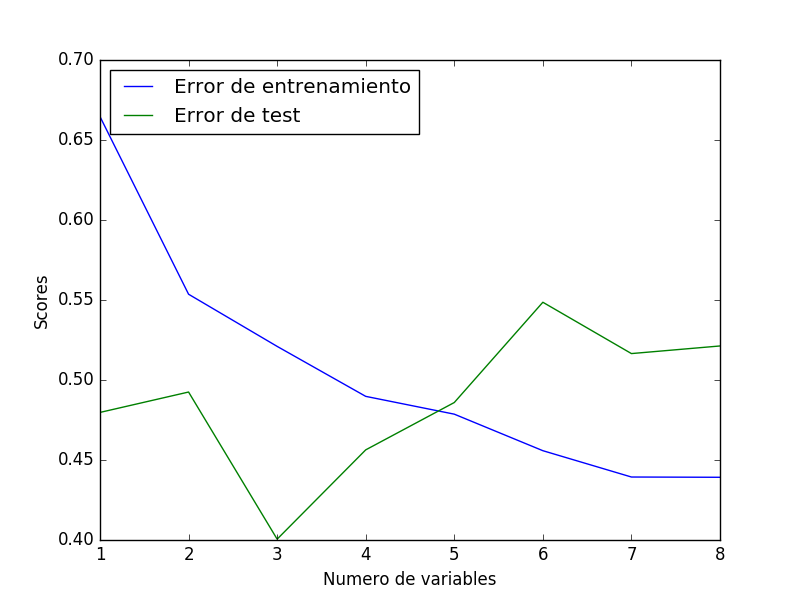
\includegraphics[width=0.6\textwidth]{Images/p2_fig1} 
=======
 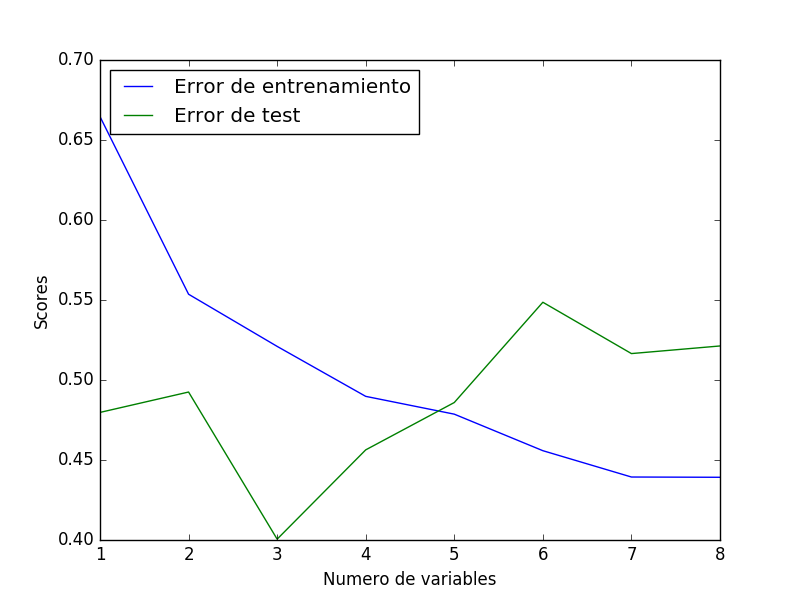
\includegraphics[width=0.6\textwidth]{Images/p2_fig1.png} 
>>>>>>> e0cf97e56a517f5af7fea26cfb70cdea0aed1267
  \caption{Error de entrenamiento vs error de test para Forward Step-wise
    Selection. A simple vista se puede observar un valor óptimo donde conviene
    dejar de seleccionar variables. }
  \label{fig:p2_g1}
\end{figure}

En la imagen se muestra un patrón de subajuste y sobreajuste a medida que se
aumenta el numero de variables. El error de entrenamiento siempre cae como es
esperado, pero el error de test parte siendo menor al de entrenamiento, pero al
escoger más variables sube también su error. En este caso, después de 5
variables no conviene escoger mas variables porque se produce mucho sobreajuste.

\subsection{Backward Step-wise Selection}

El algoritmo \textit{Backward Step-wise Selection}(BSS) funciona de forma
similar a FSS, excepto que parte con un modelo hecho con todas las variables, y
se van quitando una a una, escogiendo la que esté con peor puntaje que el resto.\\

La implementación es similar a FSS. También se usó zscore para calcular quién
debe dejar el conjunto de variables, pero en este caso, se escogió a los que
peor salieron evaluados.\\


El orden de selección de atributos es exactamente el mismo que en FSS pero
invertido. Ésto es esperado, ya que la forma de ordenar a las variables es la
misma pero se selecciona el peor en vez del mejor.

El comportamiento en general en éste dataset es similar en ambos casos, lo cual
se puede confirmar con su gráfico asociado.

\begin{figure}[H]
  \centering
<<<<<<< HEAD
 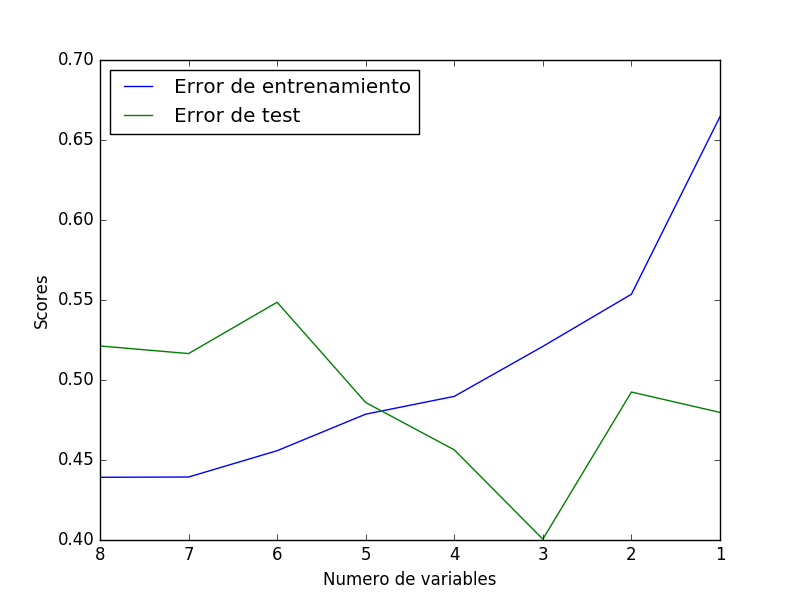
\includegraphics[width=0.6\textwidth]{Images/p2_fig2} 
=======
 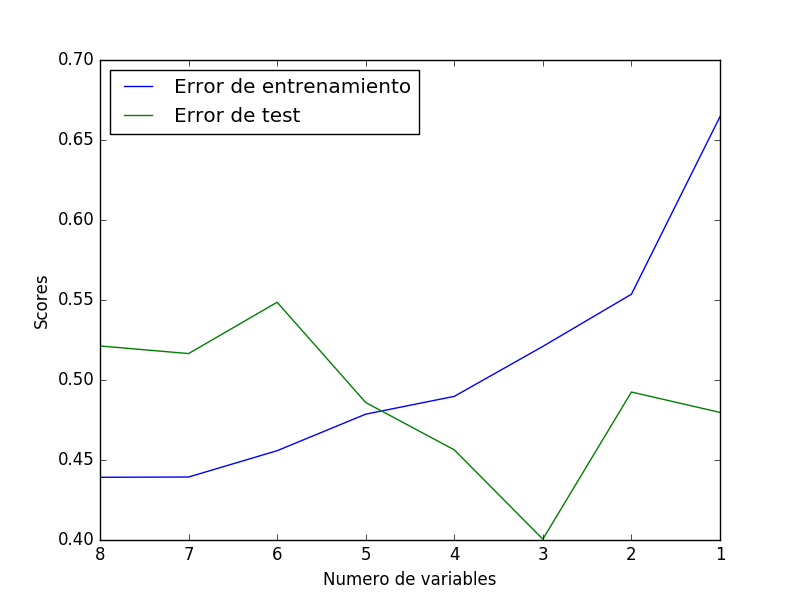
\includegraphics[width=0.6\textwidth]{Images/p2_fig2.png} 
>>>>>>> e0cf97e56a517f5af7fea26cfb70cdea0aed1267
  \caption{Error de entrenamiento vs error de test para Backward Step-wise
    Selection. Tiene el mismo comportamiento que FSS.}
  \label{fig:p2_g2}
\end{figure}
\section{Regularización}

\subsection{Ridge Regression}
\textit{Ridge Regression} es un método de regularización para modelos
lineales.\\

Notar que en éste tipo de regresión los cálculos se hacen más fácil de obtener,
al menos en forma conceptual, si se procede a centrar los datos usando su media.
En el código no se asume que los datos fueron centrados, por lo que al asignar
\texttt{fit\_intercept=True} a los modelos, éstos también asumen que los datos no
se centraron, por lo que hace el calculo del intercepto además del resto.


Es por lo último que se tiene que quitar del dataframe la columna
correspondiente al intercepto, porque la función Ridge va a hacer su ``fit''
como si dicha columna fuera un dato más, lo cual no es conveniente.\\


En el trabajo se aplicaron parámetros de regularización en el rango de $\lambda
\in [10^4,10^-1]$ mediante una escala logarítmica. Los resultados están resumidos
en el siguiente gráfico:

\begin{figure}[H]
  \centering
<<<<<<< HEAD
  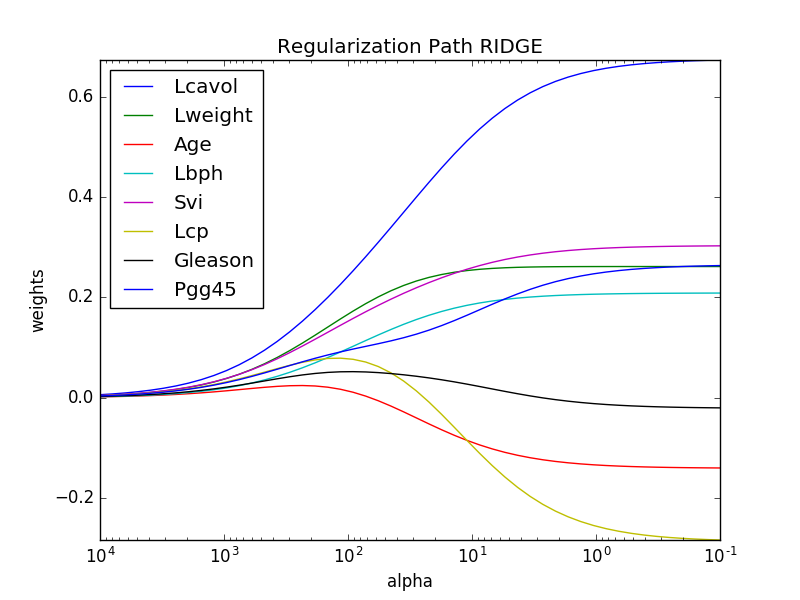
\includegraphics[width=0.6\textwidth]{Images/p3_fig1} 
=======
  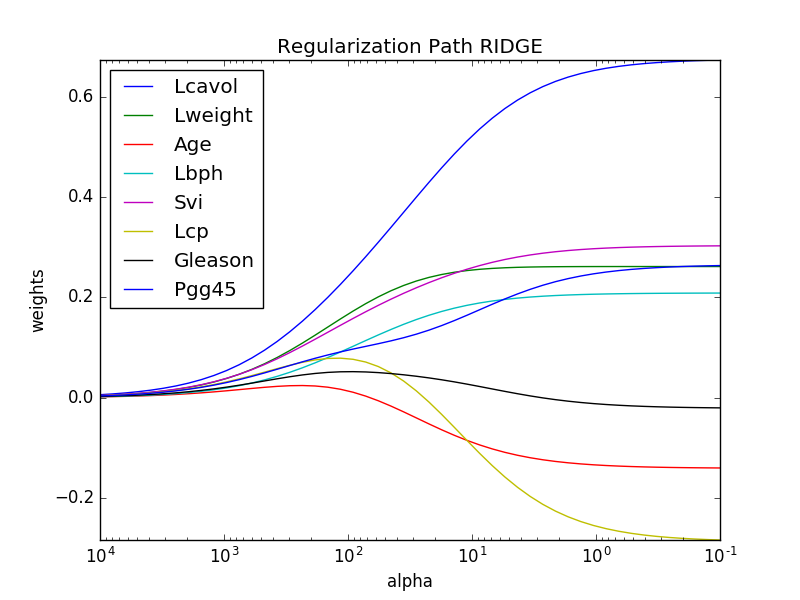
\includegraphics[width=0.6\textwidth]{Images/p3_fig1.png} 
>>>>>>> e0cf97e56a517f5af7fea26cfb70cdea0aed1267
  \caption{Gráfico del camino de regularización de Ridge Regression. A medida
    que disminuye $\lambda$ se obtiene una mayor diferenciación entre cada atributo.}
  \label{fig:p3_g1}
\end{figure}

Al disminuir el parámetro de regularización se vé como los pesos de cada
atributo empiezan a diferenciarse más. Con $\lambda$ más grande los atributos
empiezan a converger a un mismo peso.
\subsection{Lasso Regression}
\textit{Lasso Regression}hace el mismo trabajo que Ridge, pero también tiene
funciones en reducción de variables.\\

Ocupando un $\lambda \in [10^1,10^-2]$ en escala logarítmica, se generó el
siguiente gráfico para Lasso:


\begin{figure}[H]
  \centering
<<<<<<< HEAD
  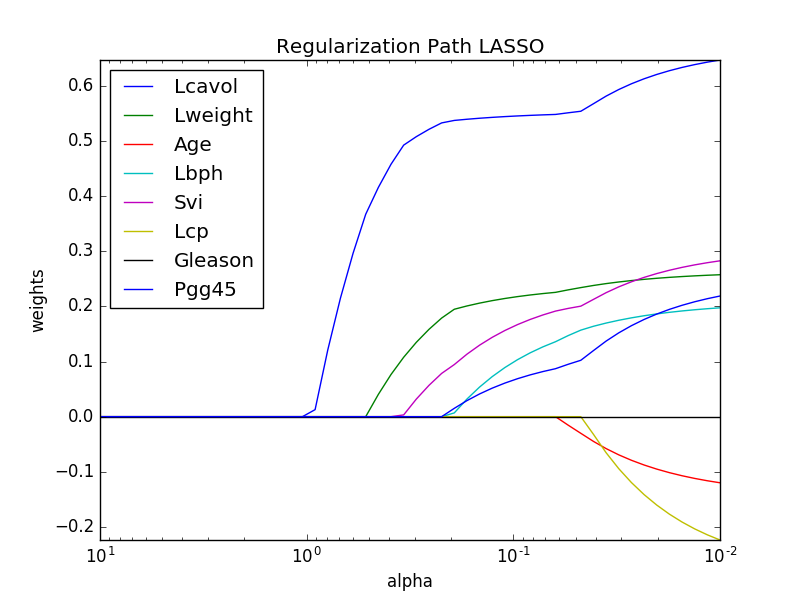
\includegraphics[width=0.6\textwidth]{Images/p3_fig2} 
=======
  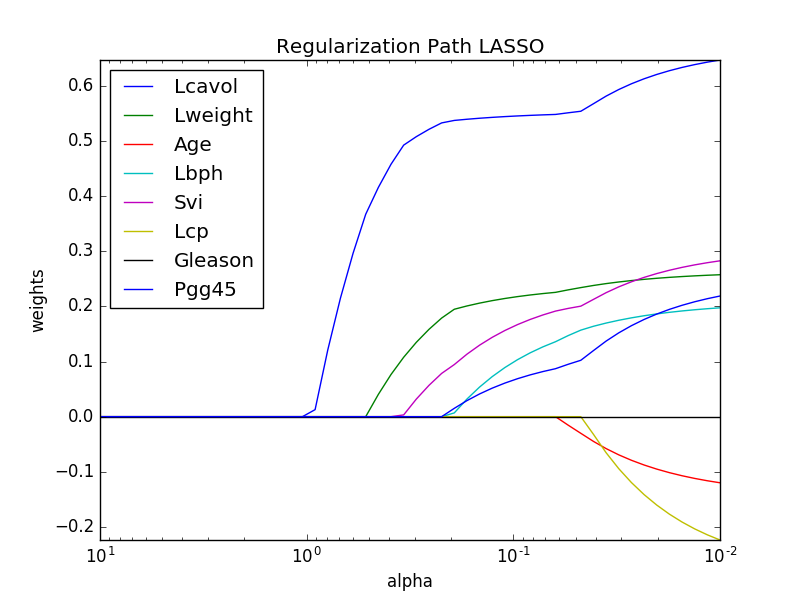
\includegraphics[width=0.6\textwidth]{Images/p3_fig2.png} 
>>>>>>> e0cf97e56a517f5af7fea26cfb70cdea0aed1267
  \caption{Gráfico del camino de regularización de Lasso Regression.}
  \label{fig:p3_g1}
\end{figure}

A diferencia de Ridge, Lasso directamente elimina variables a medida que aumenta
su $\lambda$. En el caso anterior con valores de regularización altos igual
habían trazas de variables que en realidad son insignificantes. En el caso de
Lasso las variables que menos aportan son sistemáticamente hechas cero, llegando
un punto donde no todos los atributos tienen peso nulo.

\subsection{Error de pruebas de Ridge Regression}
El error de pruebas obtenido para Ridge Regression se encuentra en el gráfico
siguiente:

\begin{figure}[H]
  \centering
<<<<<<< HEAD
  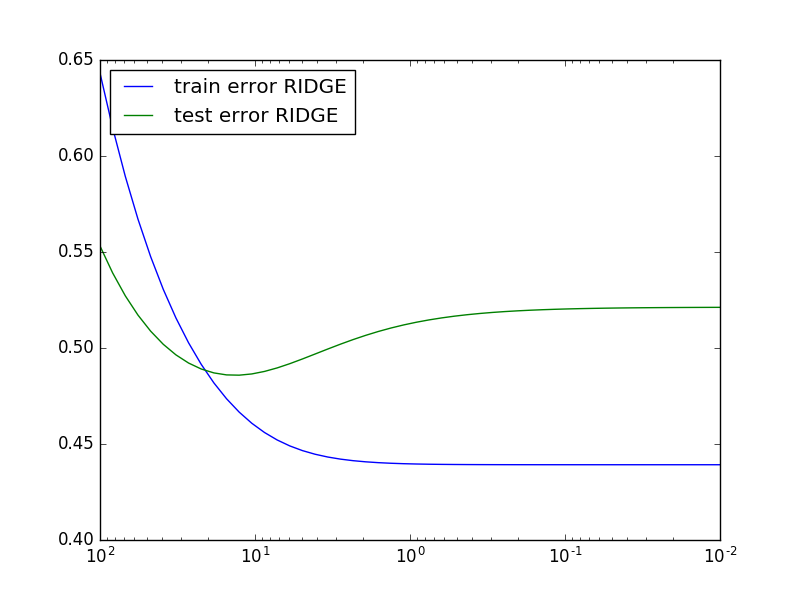
\includegraphics[width=0.6\textwidth]{Images/p3_fig3} 
=======
  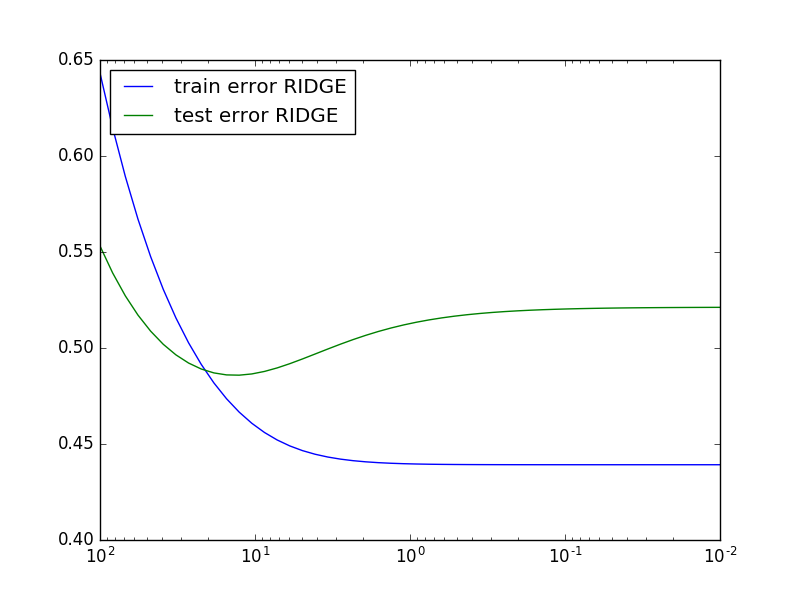
\includegraphics[width=0.6\textwidth]{Images/p3_fig3.png} 
>>>>>>> e0cf97e56a517f5af7fea26cfb70cdea0aed1267
  \caption{Error de pruebas vs error de entrenamiento para RIDGE. Se puede
    observar el patrón de sobre y subajuste.}
  \label{fig:p3_g2}
\end{figure}

Se puede observar que el punto donde ambos errores son iguales está entre 10 y
100. Si se trata de escoger $\lambda$ usando éste criterio se debería considerar
mejor escoger un valor superior a 10 para evitar el sobreajuste.
\subsection{Error de pruebas de Lasso Regression}
Los errores de entrenamiento y pruebas para Lasso Regression se encuentran
resumidos en el siguiente gráfico:

\begin{figure}[H]
  \centering
<<<<<<< HEAD
  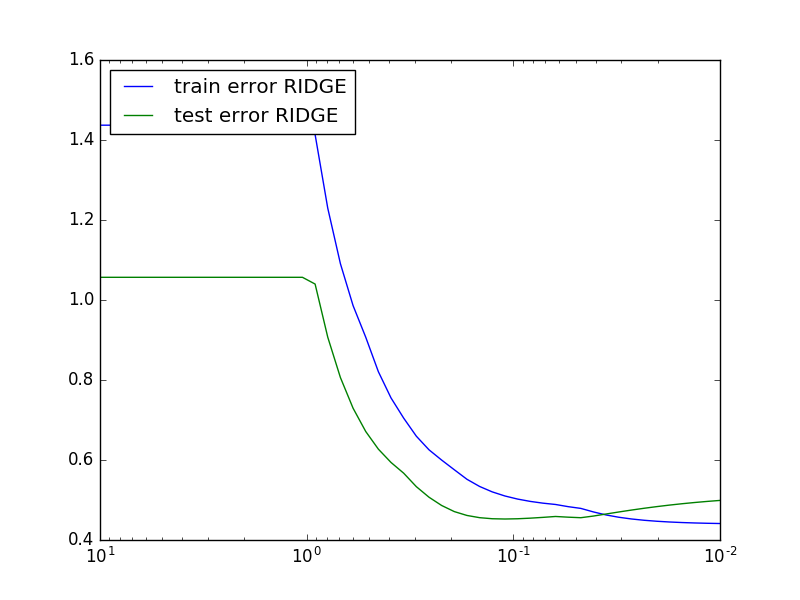
\includegraphics[width=0.6\textwidth]{Images/p3_fig4} 
=======
  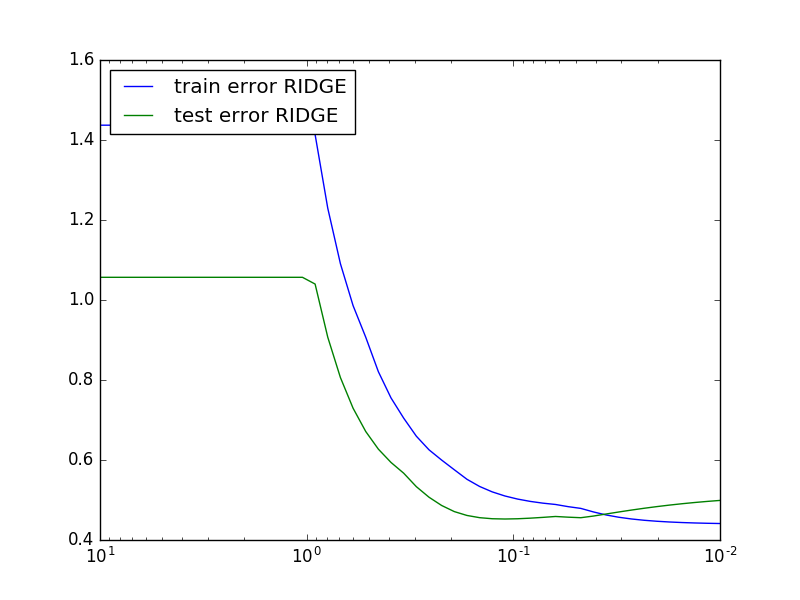
\includegraphics[width=0.6\textwidth]{Images/p3_fig4.png} 
>>>>>>> e0cf97e56a517f5af7fea26cfb70cdea0aed1267
  \caption{Error de pruebas vs error de entrenamiento para RIDGE. Se puede
    observar el patrón de sobre y subajuste.}
  \label{fig:p3_g2}
\end{figure}

En este gráfico se puede observar que el punto donde no hay ni underfitting ni
overfitting está entre $\lambda$ igual a 0.1 y 0.01. Por otro lado, el error de
test empieza a aumentar entre 1 y 0.1.

Hay que mencionar que existe una anomalía en $\lambda = 1$. El error de
entrenamiento se mantiene constante después de ese punto, al igual que el de
test. Esto corresponde a que en ese punto todas las variables tienen peso 0, por
lo cual no hay error que medir.
\subsection{Encontrar los valores optimos para cada tipo de regularizador}
Usando los gráficos se puede tener una idea del valor óptimo, pero por el rango
no se puede dar un número exacto. Para encontrar dicho valor se usará kfold
cross validation con $K = 10$ cajas.

Para Ridge, cross validation encontró que el mejor parámetro es 2.442053 con un
$MSE = 0.751881$. Esto está en territorio de sobreajuste de acuerdo al gráfico.
Pero también es el punto donde el error de test está en su mínimo, de acuerdo al
gráfico, así que tiene sentido usar dicho valor de $\lambda$.\\

En el caso de Lasso, el resultado es exactamente $\lambda = 0.01$. Éste es el punto donde el
error de test empieza a subir. Por otra parte, a diferencia del caso anterior,
se encuentra firmemente en territorio de underfitting.
\section{Predicción de Utilidades de Películas}

Para esta sección, se trabajó con un conjunto de datos sobre películas vistas en cines de Estados Unidos durante los años 2005 y 2009. Lo que se desea predecir es el volumen de utilidades (en dólares) que se obtienen por el estreno de una película.\\

Las películas se representan a través de diversos atributos de tipo texto o metadata. Los textos corresponden a críticas realizadas antes del estreno en diversos sitios. Los metadatas están compuestos por 7 variables, como por ejemplo, cantidad de puntos en donde se proyecta la película, el género, la calificación de la MPAA, número de actores con premio OSCAR, entre otros.\\

Los datos están contenidos en archivos, los cuales se cargan a través de python guardándolos en matrices, con la finalidad de aplicar algún modelo lineal que permita predecir la utilidad con un coeficiente de determinación de al menos 0,75.\\

A continuación, se muestra una tabla resumen con los datos obtenidos con los diferentes modelos lineales que se intentó resolver el problema con un $R^2$ de al menos 0,75.

\begin{table}[!hbt] 
\begin{center}
\begin{tabular}{| r | c | c |} 
\hline
\textbf{Modelo Lineal} & \textbf{$R^2$}\\ 
\hline 
Lineal Regression & 0.182\\ 
Ridge Regression & 0.590\\
\hline 
\end{tabular}
\caption{Resumen con los distintos métodos utilizados.} 
\label{table:peliculas}
\end{center} 
\end{table}

De la Tabla \ref{peliculas}, se observa que el que tuvo mejores resultados, o acercándose al esperado de 0.75, fue el modelo de Ridge, utilizando un alpha de 0.2. Se intentó en primer lugar, con el modelo de regresión lineal ordinario, pero dio resultados bastante malos. También se realizó con Lasso Regression, pero con este modelo se obtenían resultados negativos. \\

Finalmente, con ninguno de los 3 modelos se pudo obtener un coeficiente de determinación superior al 0.59, por lo que Ridge Regression es el modelo que mejor funcionó.

\bibliographystyle{plain}
\bibliography{Referencias}

\end{document} 